\documentclass[11pt, fleqn]{article}

\usepackage[letterpaper, margin=0.7in]{geometry}
\usepackage{graphicx}
\usepackage{subcaption}
\usepackage{cleveref}
\usepackage{listings}
\usepackage{multicol}
\usepackage{tikz}
\usepackage{bm}
\usepackage{minted}
\usetikzlibrary{arrows}
\usepackage{wrapfig}
\usepackage{amsmath}
\usepackage{amssymb}
\usepackage[section]{placeins}
\usepackage{pgfplots,wrapfig}  
\pgfplotsset{compat=newest} 
\pgfplotsset{plot coordinates/math parser=false} 
\newlength\figureheight 
\newlength\figurewidth 
\setlength{\parindent}{0pt}
\newcommand\tab[1][1cm]{\hspace*{#1}}
\usepackage{algorithm}
\usepackage[noend]{algpseudocode}

\let\oldReturn\Return
\renewcommand{\Return}{\State\oldReturn}

\raggedbottom

\begin{document}

\begin{center}

\Large{COMP6212 Assignment 4 : Shakib-Bin Hamid 25250094 sh3g12}

\end{center}

\section{Kalman Filter}

Lets suppose a data generative process is a linear combination of its past values, i.e. the current process process parameters are a linear combination of previous process parameters. In this respect we can calculate the process parameters by minimising the least squared error between the prediction and the true values, $\bm{\omega} = (\bm{Y}^t\bm{Y})^{-1}\bm{Y}^t\bm{f}$, where $\bm{Y}$ is the input data and $\bm{f}$ is the target. But this method requires calculating a new $\bm{Y}^{-1}$ (a $O(n^3)$ operation) when we receive any new data. If the process is generating a time series data (getting data one at a time), then online updating the parameters can be incredibly costly.\\

However, it can be shown that we can calcuate new parameters without calculating a new inverse, $\bm{\omega}_n = \bm{\omega}_{n-1} + L \times (f_n - \bm{\omega}_{n-1}^t\bm{y_n})$. It means that we can calculate new parameters by updating the old parameters with the scaled prediction error on new data using the old parameters. Of course we need to assume some initial values for our parameters. But, we still do not account for any noise in our process.\\

In a Kalman Filter, we may assume a process $\bm{\omega}_n = \bm{A}\bm{\omega}_{n-1} + \bm{\epsilon}(n)$, where the process noise $\bm{\epsilon} \sim \mathcal{N}(0, \bm{Q})$. Here we can assume that our parameters are a linear transformation of previous parameters corrupted by Gaussian noise. Similarly, we can assume that our observation $f_n = \bm{\omega}_n\bm{y}_n + \xi(n)$, where observation noise $\xi \sim \mathcal{N}(0, R)$.\\

\cite{mahler} claims that we can predict the monthly S\&P 500 index using a Kalman filter. In order to verify his claim, I have implemented Algorithm \ref{alg:kalman} -

\begin{algorithm}[H]
\caption{S\&P 500 Index Prediction using a Kalman Filter}
\label{alg:kalman}
\begin{algorithmic}[1]

\Procedure{Kalman}{$\bm{s}, o, \alpha$} \Comment{$\bm{s}$ = index, $o$ = order, $\alpha$ = a constant}

\State

\State $N$ = $size(\bm{s}, 1)$; \Comment{Number of months}
\State $\bm{Y}$ = $zeros(N - o + 1, o)$; \Comment{Input data in $o$ order windows}
\State $\bm{W}$ = $zeros(N, o)$; \Comment{Weights at every point}
\State $\bm{e}$ = $zeros(N - o + 1, 1)$; \Comment{Prediction error at every point}

\State

\State $m$ = $ar(s, o)$; \Comment{Matlab's autoregression function}
\State $R$ = $m.NoiseVariance$; \Comment{Observation noise variance}
\State $\bm{w}$ = $(m.a(2:o+1) \times -1)^t$; \Comment{Current weight set to initial value}

\State

\State $\bm{A}$ = $\bm{I}_o$ \Comment{$\bm{I}_o$ is the $o$ order Identity}
\State $\bm{Q}$ = $\alpha\bm{I}_o$ \Comment{Process noise covariance}
\State $\bm{P}$ = $\bm{I}_o$ \Comment{Uncertainity or covariance of parameters}

\State

\For {$n \gets o + 1,N$}

	\State $\bm{y}_n$ = $\bm{Y}(n, :)$ = $\bm{s}(n - o:n - 1)$ \Comment{Input is last $o$ months' index}

	\State

	\State $\bm{P}$ = $\bm{A}\bm{P}\bm{A}^t$ + $\bm{Q}$ \Comment{Uncertainity on parameters increases}

	\State
	
	\State $\bm{e}(n)$ = $\bm{s}(n)$ - $\bm{w}^t\bm{y}_n$ \Comment{Prediction Error}
	\State $\bm{K}$ = $\bm{P}\bm{y}_n/(R + \bm{y}_n^t\bm{P}\bm{y}_n)$ \Comment{Kalman Gain}

	\State

	\State $\bm{w} = \bm{W}(n, :)$ = $\bm{w} + \bm{K}\bm{e}(n)$ \Comment{Correction}
	\State $\bm{P}$ = $(\bm{I}_o - \bm{K}\bm{y}_n^t)\bm{P}$ 

\EndFor

\EndProcedure
\end{algorithmic}
\end{algorithm}

\begin{wrapfigure}{!h}{0.5\textwidth}
  	\centering
  	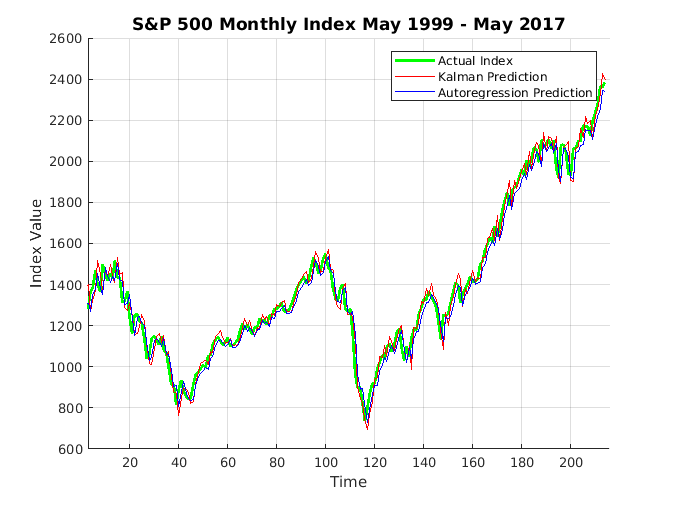
\includegraphics[width=0.5\textwidth]{kalman-autoreg-pred.png}
	\caption{Kalman \& Autoregression Prediction}
	\label{fig:kalman-autoreg-pred}
	\vspace{-1cm}
\end{wrapfigure}

The input at each point in time is past $o$ index values. Observation noise $R$ is taken as the residual variance from an autoregression model using \texttt{ar} function of Matlab's System Identification Toolbox. Process noise covariance needed to be tuned via $\alpha$. Figure \ref{fig:error-vs-alpha-order-3} (where I have plotted the cumulative sum of prediction error as a function of $\alpha$ for a 3rd order filter), indicates that $10^{-3}$ is a reasonable value for $\alpha$. Unless otherwise specified, it can be assumed that a 3rd order filter and autoregression was in use. The parameters were initialised in Line 10 and covariance in Line 14.\\

\begin{figure}[!h]
    \centering
    \begin{subfigure}[b]{0.45\textwidth}
        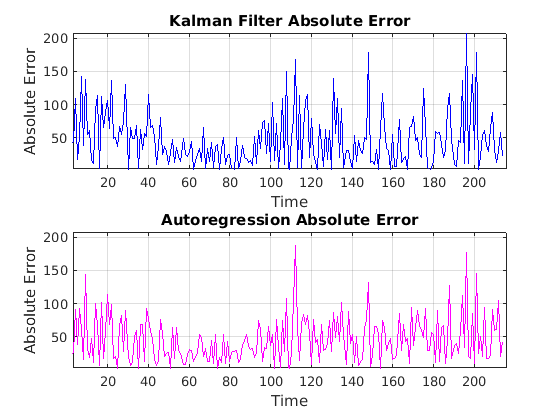
\includegraphics[width=\textwidth]{kalman-autoreg-error.png}
		\caption{Index Prediction Absolute Error}
		\label{fig:kalman-autoreg-error}
    \end{subfigure}
    ~ 
    \begin{subfigure}[b]{0.42\textwidth}
        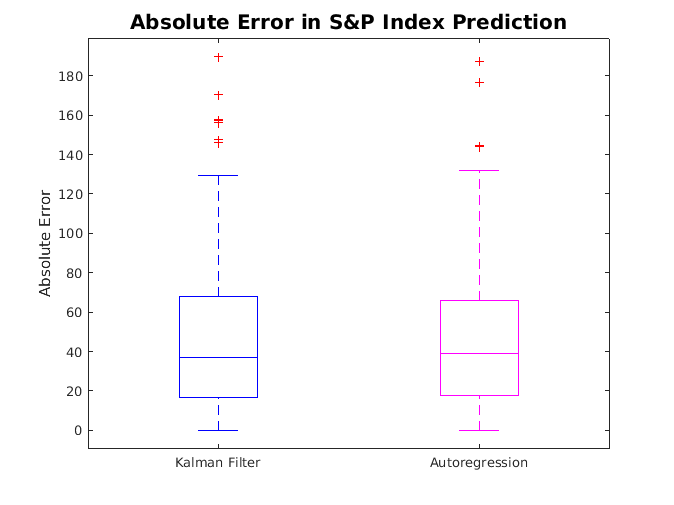
\includegraphics[width=\textwidth]{kalman-autoreg-error-boxplot.png}
		\caption{Index Prediction Error Comparison}
		\label{fig:kalman-autoreg-error-boxplot}
    \end{subfigure}
    \caption{Prediction Error}
	\label{fig:prediction-error}
\end{figure}

I began by generating an artificial time series using white Gaussian noise (Matlab's \texttt{wgn} function) and $(0.5, 0.6, 0.1)$ weights. The kalman filter quickly stabilises on this data at the expected weights (Figure \ref{fig:kalman-parameter-converge-artificial}). After confirming the correctness of the kalman filter, I applied it to real data.\\

Figure \ref{fig:kalman-autoreg-pred} is showing the monthly index values, as well as prediction made from an autoregression and the implemented Kalman filter. Clearly both are very close to the true values of the index. We can also see from Figure \ref{fig:kalman-autoreg-error} that both methods produce very similar error patterns. Figure \ref{fig:kalman-autoreg-error-boxplot} shows that the errors have very similar spread.\\


\begin{figure}[!h]
    \centering
	\begin{subfigure}[b]{0.28\textwidth}
        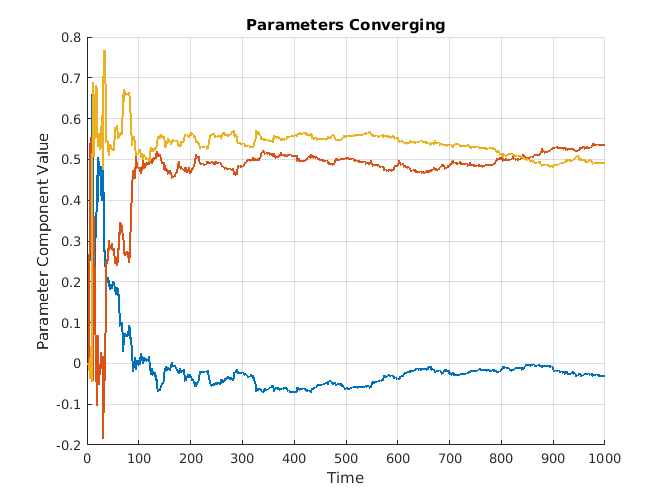
\includegraphics[width=\textwidth]{kalman-parameter-converge-artificial.png}
	\caption{Artifical}
	\label{fig:kalman-parameter-converge-artificial}
    \end{subfigure}
    ~ 
    \begin{subfigure}[b]{0.28\textwidth}
        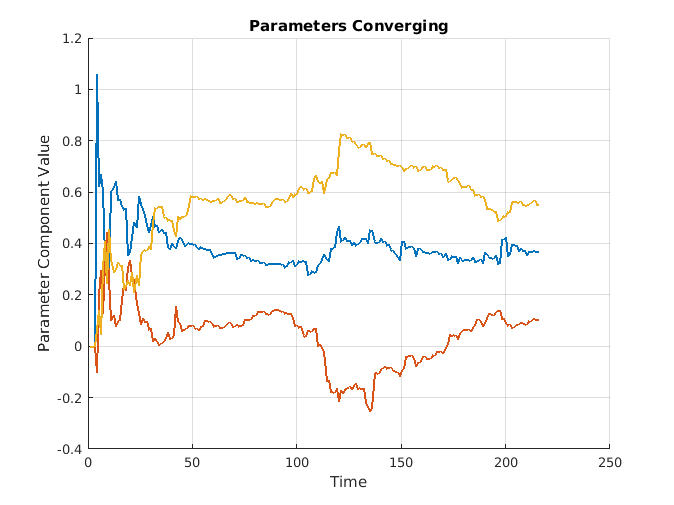
\includegraphics[width=\textwidth]{kalman-parameter-converge.png}
		\caption{$R \approx 53$}
		\label{fig:kalman-parameter-converge}
    \end{subfigure}
	~ 
    \begin{subfigure}[b]{0.3\textwidth}
        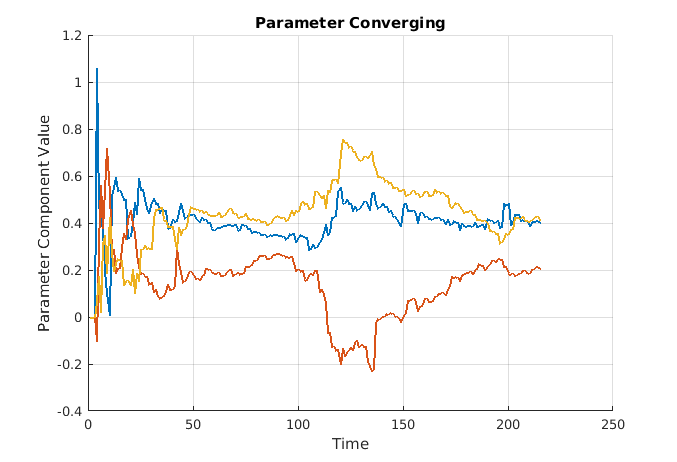
\includegraphics[width=\textwidth]{kalman-parameter-converge-r-420.png}
		\caption{$R$ = $420$}
		\label{fig:kalman-parameter-converge-r-420}
    \end{subfigure}
    \caption{Parameter Convergence}
	\label{fig:o-alpha-error}
\end{figure}

Figure \ref{fig:kalman-parameter-converge} shows the convergence of the parameters on real data. It demonstrates the recursive correction of weights.\\

\begin{figure}[!h]
    \centering
    \begin{subfigure}[b]{0.3\textwidth}
        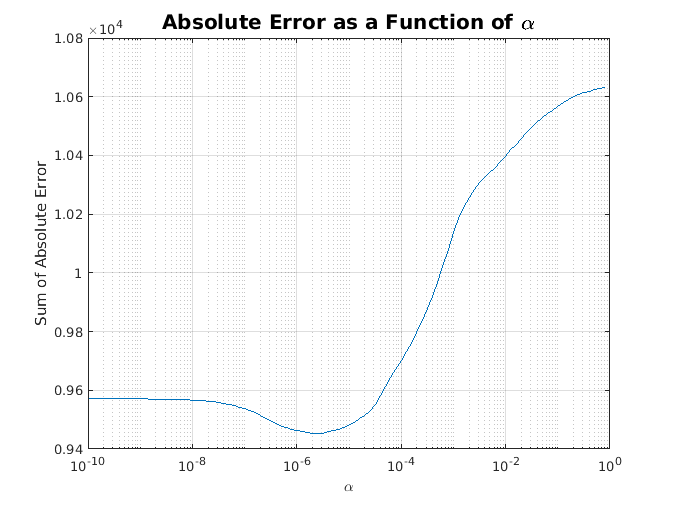
\includegraphics[width=\textwidth]{error-vs-alpha-order-3.png}
	\caption{$\bm{e}$ = $f(\alpha)$}
	\label{fig:error-vs-alpha-order-3}
    \end{subfigure}
    ~ 
	\begin{subfigure}[b]{0.3\textwidth}
        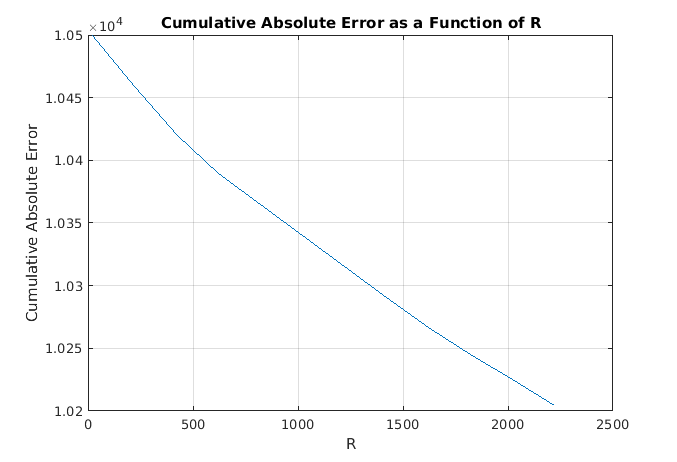
\includegraphics[width=\textwidth]{error-vs-r.png}
	\caption{$\bm{e}$ = $f(R)$}
	\label{fig:error-vs-r}
    \end{subfigure}
	\caption{Tuning $\alpha$ and $R$}
	\label{fig:tuning-alpha-r}
\end{figure}

Now we can also observe from Figure \ref{fig:error-vs-alpha-order-3} that error changes as the choice of $\alpha$ changes. The $\alpha$ choice is rather arbritrary and needs tuning. As I mentioned earlier, I chose $\alpha$ = $10^{-3}$ for all orders, since it seemed reasonable at most orders. Similarly, I plotted the error by varying $R$ = $(20:200:2000)$. Figure \ref{fig:error-vs-r} shows the effect of tuning $R$. I have chosen the noise variance of an autoregression model to be the effective $R$ after this observation.\\

\begin{figure}[!h]
    \centering
	\begin{subfigure}[b]{0.3\textwidth}
        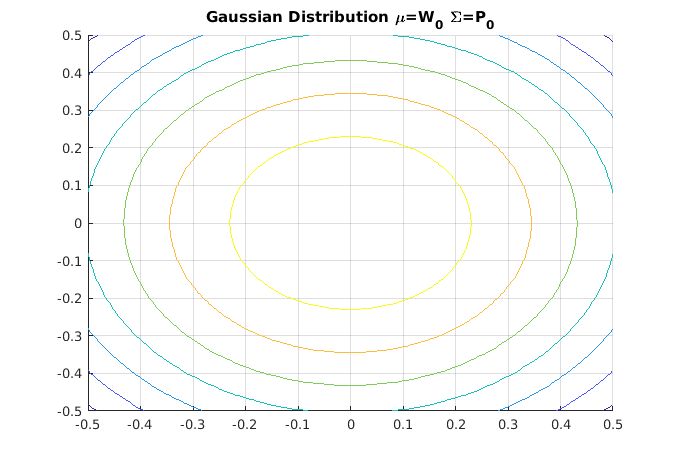
\includegraphics[width=\textwidth]{kalman-parameter-contour-initial.png}
	\caption{Initial Parameter Contour}
	\label{fig:kalman-parameter-contour-initial}
    \end{subfigure}
    ~ 
	\begin{subfigure}[b]{0.3\textwidth}
        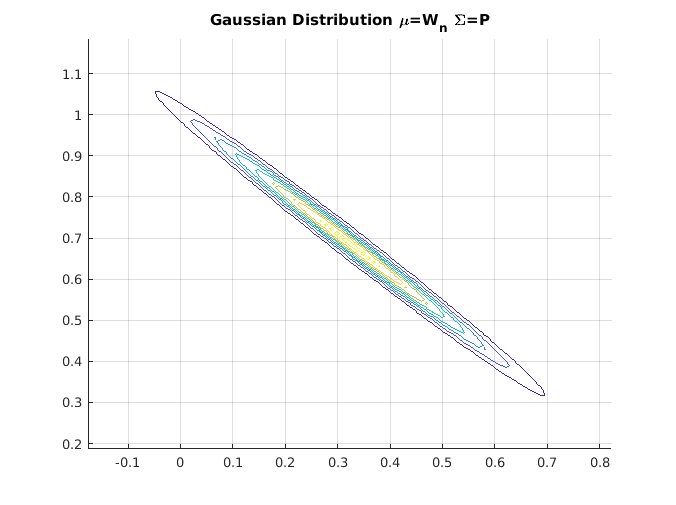
\includegraphics[width=\textwidth]{kalman-parameter-contour.png}
	\caption{Final Parameter Contour}
	\label{fig:kalman-parameter-contour}
    \end{subfigure}
	\caption{Parameter Contour Updates}
	\label{fig:kalman-parameter}
\end{figure}

Finally, from Figure \ref{fig:kalman-parameter}, we can clearly see the updates on the parameters. This diagram shows the spread of the parameters at the start and at the end of the kalman filter. We can clearly see how the spread has been shrinked into the final shape from the initial uniform shape. This is exactly as expected.\\

Overall, the benefit of building a kalman filter to deal with financial time series is that we can isolate the noise and tune the process of doing so. At the same time we receive a distribution of our solution, which tells us the confidence in the parameters. This way we may be able to make better judgements. However, we are yet to explain the residual noise.

\section{Predicting the Residual in Kalman Filter}

The paper tries to explain the residual in the Kalman filter by the following variables - S\&P 500 Price to Earnings Ratio (PER), Spot Oil Price, West Texas Intermediate (OIL), NAPM, ISM Manufacturing, Purchasing Managers' Composite Index (PMI), Disposable Personal Income (INCOME), Corporate Profits After Tax (CORP PROFIT), US Population (POPULATION) and US Unemployment Rate (UNEMPLOYMENT). The monthly data (May 1999 - February 2017) for these were collected from \cite{fed}. It was normalised via \texttt{zscore} function of Matlab's Statistics and Machine Learning Toolbox. The missing months' data were padded by the last month's data. The S\&P 500 index, Kalman Filter and Augoregression of 2nd order were also calculated. \\

\begin{figure}[!h]
    \centering
    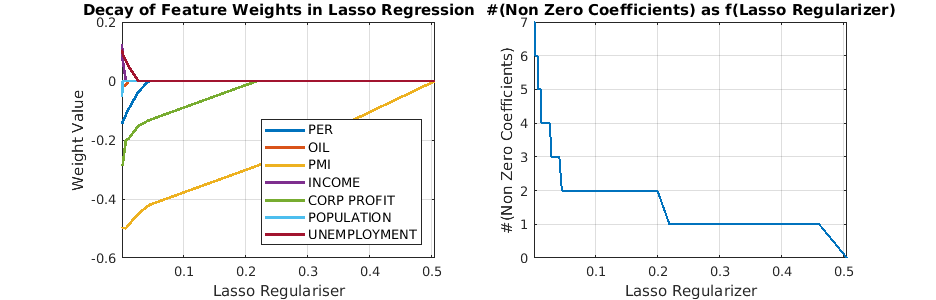
\includegraphics[width=0.8\textwidth]{decay-lasso.png}
	\caption{Decaying Features in Lasso Regulariser}
	\label{fig:decay-lasso}
\end{figure}

Matlab's \texttt{lasso} function was used to run a lasso regularisation with 5 fold validation. The input was a 7 column matrix with the features mentioned in the last paragraph. The target output was the residual from a 2nd order Kalman Filter index prediction. It ran a lasso regularisation by solving the optimisation $min_{w_0, w}(\frac{1}{2N}\Sigma_{i=1}^N(y_i - w_0 - x_i^Tw)^2 + \lambda\Sigma_{j=1}^p|w_j|)$. The optimisation was done for $\lambda$ in range of $(0,0.5)$ for 100 values. The values for $w_0$ were approximately $10^{-6}$. So, its effect can be ignored.\\

As expected (from Figure \ref{fig:decay-lasso}), the number of non-zero weights for the features reduced as $\lambda$ or the regularisation penalty increased. It seems that it was most stable for 1 or 2 features. From Figure \ref{fig:decay-lasso} left, we can see that PMI and CORP PROFIT were the last two features to be eliminated. Also, from Figure \ref{fig:error-vs-lambda} we can see that, the least error was when $\lambda$ was set to 0, i.e. we only wanted to match the target residual. As usual the choice of $\lambda$ is one of tuning. If we want the weights to be sparse (as we do), we would like to choose a $\lambda$ that will set all but 2 or 3 weights to 0.\\

\begin{figure}[!h]
    \centering
	\begin{subfigure}[b]{0.3\textwidth}
        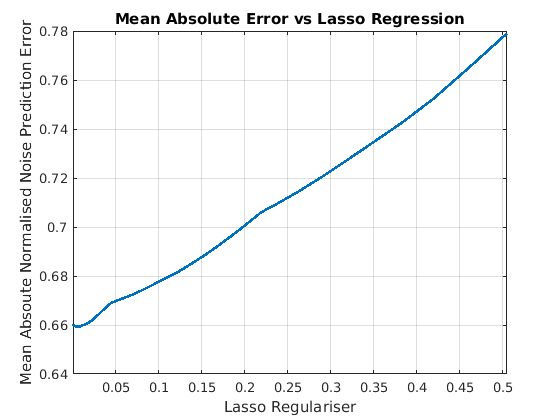
\includegraphics[width=\textwidth]{error-vs-lambda.png}
	\caption{Lambda vs Noise Prediction Error}
	\label{fig:error-vs-lambda}
    \end{subfigure}
    ~ 
	\begin{subfigure}[b]{0.3\textwidth}
        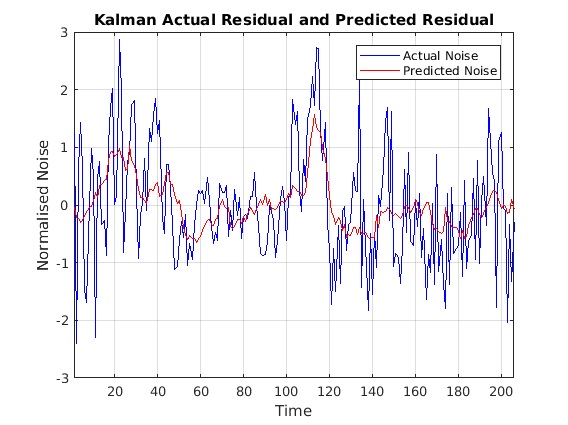
\includegraphics[width=\textwidth]{noise-prediction.png}
	\caption{Kalman Noise Prediction by Lasso}
	\label{fig:noise-prediction}
    \end{subfigure}
 	~ 
	\begin{subfigure}[b]{0.3\textwidth}
        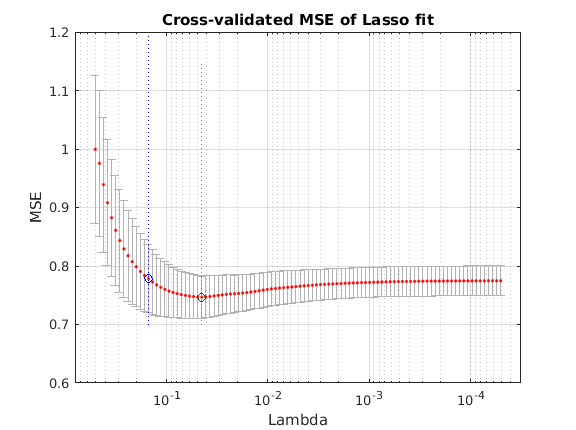
\includegraphics[width=\textwidth]{mse-lasso.png}
	\caption{Lasso Plot with Cross-Validated Fits}
	\label{fig:mse-lasso}
    \end{subfigure}
	\caption{Lasso Plots}
	\label{fig:lasso-figs}
\end{figure}

If the entire residual data is used for the lasso regression, we can fit the residual fairly well (Figure \ref{fig:noise-prediction}). I also plotted the cross validated fit in Figure \ref{fig:mse-lasso}. The blue dot is the value of $\lambda$ that gives the min MSE (Mean Squared Error). The green dot is one standard deviation away. This plot gives us an idea of how the residual prediction progressed as $\lambda$ values were changed.\\

However, our final goal is to not just to run the lasso regression on all of the residual data in one go. Just like we performed a 2nd order Kalman Filter or Autoregression, we would like to only predict the residual error by performing the lasso regularisation over the previous 2 months' features. Since at this point, we are confident that our lasso set up works and effectively predicts the residual, we only supply as input the past 2 month' features for each subsequent month from July 1999.

\begin{figure}[!h]
    \centering
    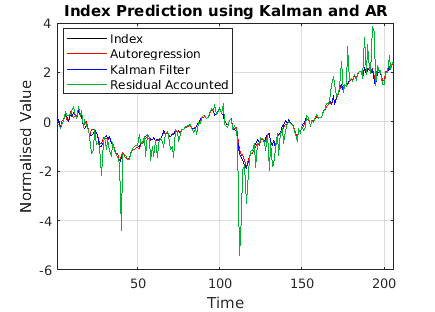
\includegraphics[width=0.5\textwidth]{laglasso.png}
	\caption{Two Months Lagged Residual Prediction Added to 2nd Order Kalman Filter Prediction}
	\label{fig:laglasso}
\end{figure}

Just as expected, the weights for the features for each month were sparse, leaving only 1-3 non-zero values - the PMI, CORP PROFIT and PER. I added the predicted residual to Kalman Filter's index prediction. Finally I plotted the actual index values and all the predictions in Figure \ref{fig:laglasso}. It still predicts fairly well. However, it has to be noted that the residual matching is sensitive around extreme times. Take the crests in time series for example. At the extremes when we see upward trends for extended periods, it does not forecast well (consider the end of the time series). This precisely coincides with the claim made in the paper. It is more prominent if we use, for each month, all previous features data as input to the lasso regularisation in Figure \ref{fig:laglasso-all}. I believe at that point the exogenous features  try to overtake the index data in the recent window, i.e. it amplifies the 'good fortune'. We would need to be cautionary in these cases.

\begin{figure}[!h]
    \centering
    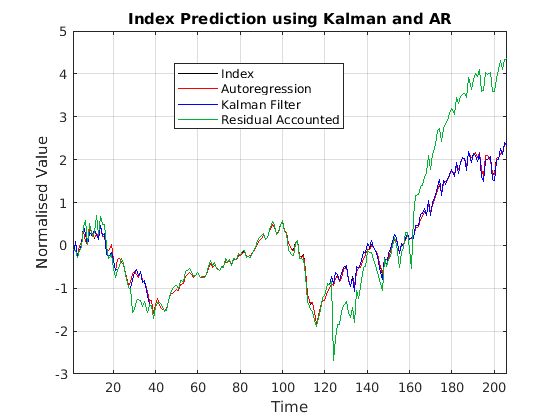
\includegraphics[width=0.5\textwidth]{laglasso_all.png}
	\caption{All Previous Months' Features are Used in Residual Forecast}
	\label{fig:laglasso-all}
\end{figure}

Finally, it can be said that we can efficiently forecast the S\&P 500 index from a recent window of previous index data. When a Kalman Filter is used, we can also try to model the residual using exogenous financial data, so that we can have more information in making financial decision. It must be said that the methods require regular tuning of certain parameters and may not work well in extreme upheavals. But it does give us a mathematical framework in efficiently explaining the financial markets. This is the point of computational finance.

\begin{thebibliography}{9}
\bibitem{mahler} 
N. Mahler, "Modeling the S \& P 500 index using the Kalman filter and the LagLasso," in \textit{Machine Learning for Signal Processing, 2009. MLSP 2009. IEEE International Workshop on, Sept 2009}, pp. 1–6.

\bibitem{fed} 
Federal Reserve Bank of St. Louis, "Economic Research," at \textit{https://research.stlouisfed.org/} [ONLINE - Last Accessed 19 May 2017].

\end{thebibliography}

\end{document}












































